\newpage
\begin{center}
\noindent\textbf{ВВЕДЕНИЕ}\label{chapters:introduction}
\vspace{1.5mm}
\end{center}

Целью настоящей дипломной работы является получение конструктивных верхних оценок для хроматического числа двумерной сферы, 
то есть построения таких раскрасок сферы, при которых точки, находящиеся на единичном расстоянии, раскрашены по-разному. 
Это задача примыкает к области классических исследований плотнейших упаковок и редчайших покрытий сфер, находится на стыке
теории графов, комбинаторной геометрии и теории кодирования.
Актуальность данной работы обусловлена отсутствием конструктивных методов получения раскрасок сфер и слабой изученностью рассматриваемой задачи, в отличие от асимптотики хроматических чисел $n$-мерных сфер при $n\to\infty$.

Для достижения поставленной цели необходимо решить следующие задачи:

\begin{enumerate}[leftmargin=1cm,topsep=0pt,itemsep=-1ex,partopsep=1ex,parsep=1ex,label=\arabic{*}.]

\item Cвести задачу о раскраске графа в $m$ цветов к задаче булевой выполнимости.
\item Провести исследование алгоритмов и методов, применяемых при построении современных \textit{SAT}-решателей.
\item Применить \textit{SAT}-решатели для поиска хроматического числа графов и получить корректные раскраски сфер, вычислить диапазоны радиусов.
\item Получить оценки хроматических чисел сфер на основе решений задачи Томсона о минимуме потенциала системы $k$ точечных зарядов на сфере и разбиений на области Вороного.
\item Доказать нижние оценки для хроматических чисел квадратов двойственных графов (триангуляций Делоне).

\end{enumerate}

Рассматриваемая задача тесно связана с классической задачей Нелсона — Эрдёша — Хадвигера о хроматическом числе $\chi(\mathbb{R}^2)$ континуального графа, вершинами которого являются точки плоскости, причем ребрами соединены вершины, находящиеся на единичном евклидовом расстоянии. Иными словами, требуется раскрасить плоскость в конечное число цветов так, чтобы точки, находящиеся на единичном расстоянии, имели разный цвет. Какое наименьшее число цветов для этого потребуется? В настоящее время известно, что $5 \leq \chi(\mathbb{R}^2) \leq 7$. Если вторая оценка тривиальна и основана на раскраске гексагонального замощения (\figurename{ \ref{introduction:fig:plane}}), то оценка снизу была получена Хойле [\ref{bib:Heule2018}] лишь в 2018 году при помощи компьютерных вычислений. 

\begin{figure}[h]
\centering
\captionsetup{justification=centering}
\center{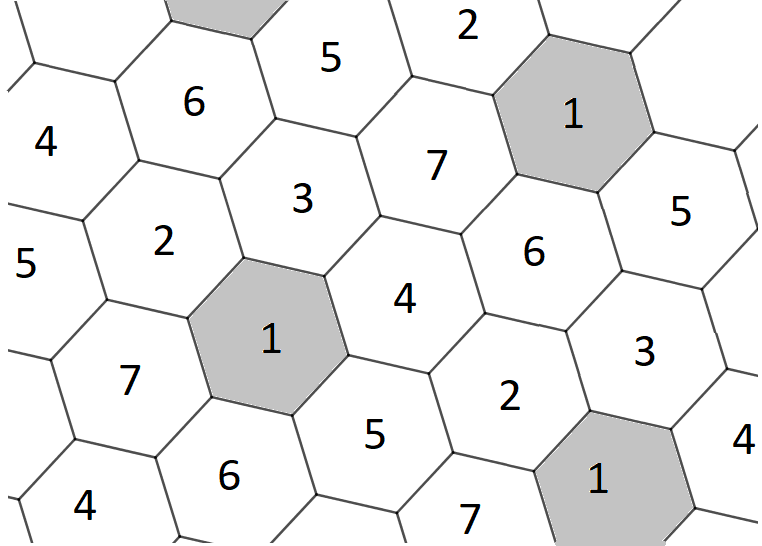
\includegraphics[width=0.4\paperwidth]{chapters/introduction/plane.png}}
\caption{Раскраска плоскости в 7 цветов.}
\label{introduction:fig:plane}
\end{figure}

Аналогичную задачу можно поставить для произвольного метрического пространства. Известно, что 
$6 \leq \chi(\mathbb{R}^3) \leq 15$ [\ref{bib:Nech}, \ref{bib:Coul}], 
получены ряд оценок для $\chi(\mathbb{R}^n)$ при $n \ge 3$, а также асимптотика $\chi(\mathbb{R}^n)$ при $n\to\infty$: 
$(1.239...+o(1))^n\leq \chi(\mathbb{R}^n)\leq (3+o(1))^n$ [\ref{bib:Rai1}, \ref{bib:Larm}].
Также рассматривались хроматические числа рациональных пространств $\mathbb{Q}^n$, многомерных сфер $S^n(r)$, 
множеств вида $\mathbb{R}^2 \times \left[ 0,~\varepsilon \right]^{k}$, ограниченных множеств, точек плоскости с координатами, принадлежащими некоторому квадратичному расширению $\mathbb{Q}$ и так далее. Как правило, полагают, что расстояние между точками множества индуцировано евклидовой метрикой $\mathbb{R}^n$. Основополагающим результатом в данной области является следующая теорема [\ref{bib:BruijnErdos}].


\begin{theorem1}[Эрдеш-де Брейне]
Если $G$ — граф с множеством вершин произвольной мощности, и $\chi(G) = k$. Тогда найдется конечный подграф  $\widetilde{G} \subseteq G$, для которого $\chi(\widetilde{G}) = k$. 
\end{theorem1}

Это означает, что наилучшую из возможных оценок хроматического числа снизу всегда можно обосновать, перебирая подграфы с конечным числом вершин. Препятствием для осуществления такого перебора (даже в случае $\mathbb{R}^2$) является, во-первых, комбинаторный взрыв, а во-вторых, отсутствие методов, позволяющих раскрасить континуальный граф в тех случаях, когда критический подграф (предположительно) найден.

Отдельный класс задач возникает в том случае, если на раскраску накладываются дополнительные условия, например, измеримость каждого из множеств, раскрашенных в один из цветов. Еще более жесткое ограничение — выпуклость компонент связности одноцветных подмножеств, для плоскости — раскраска многоугольных областей. Тогда для раскраски двумерного гладкого многообразия, удовлетворяющего определенным условиям, требуется не менее 7 цветов [\ref{bib:Soifer},\ref{bib:Kronk}].